\chapter{Local Training}

\section{Local Training vs. Cloud Training}
One of the major drawbacks of using the DeepRacer in a learning environment are the costs of training. Amazon offers easy, albeit functionally limited ways of training RL models in their cloud services. This sort of contradicts the intended use, as the DeepRacer is supposed to offer a simple and affordable entry into the ways of machine learning.
 In order to circumvent this cost barrier we -- like others before us -- began setting up a training environment on one of the more powerful computers in the robotics lab. After searching the internet we found a very cost efficient method, to train the model on our own computer. Given that in our robotics-lab we gain access to a "super-computer", which would train our models easily and fast we decided to train it by ourselves. Amazon doesn't provide a easy to use interface to download and upload models because they don't want to support you using your own servers and computers to train. Following this idea it seems that a lot of people worked their way around and made their own GUI's and interfaces.
 The setup for local training is available on GitHub 

\subsection{Prerequisites}
\footcite{https://github.com/aws-deepracer-community/deepracer}. In order to function properly the computer had to meet the following requirements:

\begin{itemize}
 \item Docker + Docker Compose
 \item vncviewer 
 \item Nvidia CUDA/cuDDN 
 \item Minio
 \item Python
\end{itemize}

\subsection{Docker}

\subsubsection{Docker}
Docker is free to use software which isolates applications using container virtualisation. It simplifies application deployment because the container containing all the necessary packages, and package dependencies, can be easily transferred and mapped into a so-called Docker image. The container ensures that the resources used on the computer are separated and managed. This includes: code, runtime-modules, system tools, system-libraries etc.\repeatfootcite{Docker-Compose}

\subsubsection{Docker-Compose}
Compose is a tool used, to handle multiple Docker images. Using a YAML-File you can configure all the services a application needs. Then with only one command, you can start all your files and services from the configuration.

\subsubsection{YAML}
YAML, a super-set of JSON, is a human-readable language used for serialisation of data. Its most common use is in data files, in which data is stored and transmitted to an application. It targets the same communication applications as the Extensible Markup Language(XML). \repeatfootcite{YAML}

\subsection{VNC-Viewer}

\subsubsection{VNC}
In computing, virtual network computing (VNC) is a platform independent, graphical desktop sharing system that uses the remote frame buffer protocol (RFB) to remotely control another computational system. You differentiate between a VNC-Client and VNC-Server, multiple Clients can connect to the same server.

\subsubsection{RFB}
The Remote Frame-buffer Protocol(RFB) is a TCP Network-protocol using the Port 5900 + Desktop Number. Its main Task is to transfer data such as screen-contents and user-inputs.\repeatfootcite{RFB}

\subsubsection{VNC-Viewer}
VNC-Viewer is the Program, which allows the Client to connect to a server and remotely control it. On the other site, the server will run a VNC-Server application.\repeatfootcite{VNC/VNC-Viewer}


\subsection{Nvidia CUDA/CUDDN}

\subsubsection{CUDA}
CUDA (previously known as Compute Unified Device Architecture) is a programming technology developed by Nvidia that allows part of the program to be processed by a graphics processing unit (GPU). Providing additional computing power in the form of GPU is necessary,in a highly parallelisable program sequence (high data parallelism), because the GPU is usually much faster than the CPU. CUDA is mainly used for scientific and technical computing. CUDA is usually programmed in C, although multiple wrapper for other languages like Ruby, Python or Java exist.\repeatfootcite{Nvidia-CUDA}

\subsubsection{cuDDN}
Nvidia cuDDN(CUDA Deep Neural Network) is a library that's used for GPU accelerated deep neural network learning. It provides highly optimised implementations for routines, like pooling, forward and backward convolution, normalisation and activation layers.\repeatfootcite{Nvidia-cuDDN}

\subsection{Minio}
Minio is a popular High Performance open source-based object storage server.It's optimised to be used with Amazon S3 cloud storage service. You can use it to build a performance-based infrastructure for machine learning, application data workloads and analytics. If you want more control over the object storage server, you can also configure applications that are configured to communicate with Amazon S3 to make Minio a alternative to Amazon.

\subsection{Python}

\subsubsection{Why use Python?}
All the Amazon services provide an API that is used to communicate between them. Python3 is used in all scripts to build an establish a connection and handle the user defined functions. The Artificial Intelligence itself is also coded in Python. Therefore its the easiest and quickest way to write Code an extend the existing Codebase in Python. The rising number of Machine Learning Library's for python is one of the key points why Amazon decided to code in this language.

\subsubsection{Python}
Python is a low level Programming-Language used in many different use-cases. Its easy to learn and has a very good documentation. You have to preinstall it, because the local training solutions are all coded in Python. Its easy to read and understand if you have a big file and it also keeps the line numbers short.\repeatfootcite{Python}

\section{Amazon tools}
To train and create the model according the rules, you have to use the programs provided by Amazon. The major tools we used in our project were:

\begin{itemize}
    \item Sagemaker
    \item Robomaker
    \item S3
\end{itemize}

\subsection{Amazon Sagemaker}
Sagemaker is a service amazon provides, to create, train and handle machine learning models. It handles the normally complicated  learning process to make it easier, training multiple large models and don't have to worry about all the tools and work processes that need to be done to learn efficient. Sagemaker contains a large tool-set to handle all different components of machine learning. It also include a debugger and pro-filer, which helps identifying training-errors and performance-issues.
\newline Sagemaker Studio is a web-based visual user interface that provides you full access, control and insight of all the steps that need to be done to create train and analyse a model. You can upload own models and analyse results, make experience or provide it to get into production. 
\newline Sagemaker Data Wrangler reduces the time required to prepare Data for Machine Learning. It provides easy access to Data-preparation-workflows including data-visualisation, data-adjustment and data-exploration.
\newline Sagemaker Ground on the other side, handles all the quick and easy to use data that is needed to train a model properly. Because a model is only as good as the data that is given to it, with Sagemaker ground you are able to manage all the training data.
\newline Sagemaker Edge Manager enables you to optimise, protect, monitor, and maintain machine learning models on edge device clusters to ensure that the models deployed on edge devices work properly.\repeatfootcite{Sagemaker}

\subsection{Amazon Robomaker}
Robomaker is a Cloud solution provided by amazon to create, simulate and test robot-based applications in large amounts. It provides access to a fully scale-able simulation infrastructure for all you robots and your CI/CD-Integration. Your are also given access to an IDE to develop new Robot applications and ROS(Robot Operating System) extensions to make your robot collaborate with the operating System.Robomaker also provides extensions to a lot Amazon Cloud Services like Kinesis(used to Stream Videos), Polly(Speachrecognition) and Cloud Watch(Monitoring and logging) for users that use ROS. It includes a lot of Example Applications that allow an easy and quick Access. Using the AWS-Services you are able to develop complete solutions that include powerful machine learning, voice recognition and speech processing capabilities and integrate them in Robot-applications.\repeatfootcite{Robomaker}

\subsection{S3}
Amazon Simple Storage Service is a data Storage solution on whom you are able to store any kind of objects. It provides a high level of security, scale ability and performance. You can use s3 for a large variety of different use cases such as websites, mobile applications, IoT and Big Data Analytics. You are able flexibly scale your storage resources to meet fluctuating demands - without upfront investment or resource acquisition. With S3 you save money without sacrificing performance by storing data in storage classes that support different levels of data access at appropriate fees.Your data is saved via encryption functions to provide the access management of unauthorised access. Access Point facilitate the data-management access with specific permissions for your applications using a shared data set. Using specific Data-Requests you are able to make Big-Data-Analyses over all your stored S3 Objects.\repeatfootcite{s3}

\section{Other Tools}
These two Tools are getting installed automatically if you run the init.sh Script as explained below. The most important two are Gazebo and rviz.

\subsection{Gazebo}
Gazebo is an 3-Dimensional open source Robotics and Physics Simulator. It integrates the ODE Physics engine, OpenGL rendering ans supports also sensor and actuator control. Gazebo uses multiple high-performance realistic physics engines like Bullet. It provides environment rendering like lighting, shadows and textures.\repeatfootcite{Gazebo} 

\subsection{rviz}
ROS(Robot Operating System) Visualisation (rviz) is graphical user interface which outputs images and videos. In this use-case it acts as the Visual Component on which you can see the training progress and the Deepracer. Gazebo simulates the Progress and the Physics and then sends the processed output to rviz which shows the video-stream. This is very useful, because you can see a livestream from the virtual Deepracer and its training progress. Based on this you can adjust the hyperparameter to get better performance.\repeatfootcite{rviz}

\section{Implementing the local training methods}

\subsection{Deepracer-Wiki}
Although most of the Information about the Deepracer and The Amazon Deepracer League is in the Online Management Console of Amazon, some users made an own independent Deepracer-Wiki, in which you find a lot of information for local training, parameter adjustment and vehicle hacking. It also links to a community-blog, a community-website and a general community-GitHub-page. \repeatfootcite{Deepracer-Wiki}

\subsubsection{Local-Training Solutions}
The Wiki includes a total list of 6 different documented GitHub projects from users, who tried to locally install all the amazon services and set up a whole local training environment. In our installation process we tried two different Repository's, because we couldn't get the first one to work on our PC. More Information about the process will be in the next section.

\subsection{First Approach}
Our first approach was to clone a GitHub repository, who implemented the whole algorithm and a graphical user interface. The author of this project relies heavily on another repository from the GitHub user crr0004. Because his instructions were unclear and the project itself was lacking features and had poor usability, he decided to expand the project and make it easier to use. 
Before getting started with installing the tools needed to run it on your machine you have to check if your computer meets the prerequisites:
At first you have to ensure that your operating system is Ubuntu 18.04 or higher, because some of the packages needed are only available on Linux.
The next main point is that your system has to run on a Nvidia GPU and have CUDA/CUDNN installed and configured. If your machine doesn't provide a Nvidia GPU you are only able to train on your CPU which is much slower and takes a lot of time.
You also should have installed Docker as well as the Nvidia-Docker runtime. This is needed for the training environment to gain access to the GPU and create new timelines.
Lastly vncviewer has to be installed, because its the program that controls all interaction between the graphical user interface and the controllers from amazon.
If your system meets all the requirements above you have to clone to run the init.sh script.
This may take up to 10 minutes and all it does is, it clone crr0004's\repeatfootcite{Local-Training-1} repository, runs the required scripts and creates the necessary folder structure including all the needed files, to manually adjust your code, train your model, and upload it to amazon.
After the installation and initialisation process is completed, we were able to start a training session but after about 10 minutes the program crashed with a python buffer overflow. Searching the internet we did not find any evidence, that we made errors during the installation process and we also were not able to fix it.

\subsection{Final Approach}
Our second try was to download Matt Camps\repeatfootcite{Local-Training-2} solution, which also relies heavily on crr0004's GitHub repository, but it has more detailed instructions and doesn't use as much self programmed scripts.The only Prerequisites you have to have installed on your computer are the Nvidia CUDA drivers and docker compose. That made it easy, to install and debug if error occurred. The next step was to clone the Repository and run the init.sh. Although following the tutorial we were not able to start a training session. After debugging and logging we found out, that the project heavily relies on Amazon Sagemaker, but the corresponding docker image was never pulled and installed. After downloading it, the scripts ran flawlessly and no following errors occurred.

\section{Training and setup process}

\subsection{Installation Guide}
After our successful installation i am going to explain the complete installation process. \newline Before the beginning you have to have all the prerequisites installed.\repeatfootcite{Local-Training-2}

\begin{enumerate}
    \item At first set the docker-nvidia2 as the default runtime in your daemon.json file that's located in /etc/docker/ . You will find the argument \textsl{default-runtime} which you set to \textsl{nvidia} 
    \item The next step is to install Amazon Sagemaker. Use the Command \textsl{sudo apt-get install Sagemaker}  to download it from the Ubuntu packet-manager. This is necessary, because the following code will depend on the provided API from the Package.
    \item Completing the installation clone the GitHub Repository\url{https://github.com/mattcamp/deepracer-local/} and run the \textsl{start-training.sh} Script.
\end{enumerate}


\subsection{Folder structure}
In the Main-Folder, called deepracer-local are all files needed, to train the model.
The most important scripts are:

\begin{itemize}
    \item start-training.sh
    \item stop-training.sh
    \item delete-last-run.sh
    \item upload-current.sh
    \item mk-model.sh
    \item local-copy.sh
\end{itemize}

\subsubsection{start-training.sh}
Starts a new Training-Session. The model data directory must be empty, because the current progress is saved there. If you want to use a pretrained model, you have to set "pretrained": "true" in hyperparams.json. When starting for the first time, it will download 10GB of docker-images, therefore it will take a while to start the training process.

\subsubsection{stop-training.sh}
Stops the Training. If running, it will take at least 20s to stop, because it will first stop Sagemaker, then it sleeps till Robomaker creates a model.tar.gz in which the model data from the current model is stored and then it will stop completely. In this Format it is ready to be uploaded on a physical deepracer.

\subsubsection{delete-last-run.sh}
Clears the current bucket to prepair the model data directory, to start a new training session.

\subsubsection{upload-current.sh}
Loads current model files into a Model directory, that the user can specify before.

\subsubsection{mk-model.sh}
Creates a complete model from the training model, that can be uploaded to a physical car.

\subsubsection{local-copy.sh}
Copies the current trained model data to a save directory. This command has to be executed before the delete-last-run.sh script, otherwise all model data will be lost.

other important files that change regularly are:

\begin{itemize}
    \item hyperparams.json
    \item config.env
    \item custom-files directory
    \item reward.py
\end{itemize}

\subsubsection{hyperparams.json}
Includes the Hyperparameters that can be changed, such as batch-size, loss-rate and number of epochs.

\subsubsection{config.env}
Stores the Training Parameters and the track name. The track name has to be the same as in the training-params.yaml file.

\subsubsection{reward.py}
Stores the reward function, that can be changed by the user. This is most important file and is changed the most.

\subsection{starting a training session}
If you want to start a new session you have to decided between creating a new model within the session or pretraining an old one and improving the performance. 
\newline If you create a new model you have to run delete-last-run, than start-training. This will output the current training parameters and number of epoches.
\newline If you decide to train an older model you have to run local-copy before and change the "pretrained" parameter in the hyperprams.json to true and than follow the instructions as explained above.

\begin{figure}[H]
    \centering
    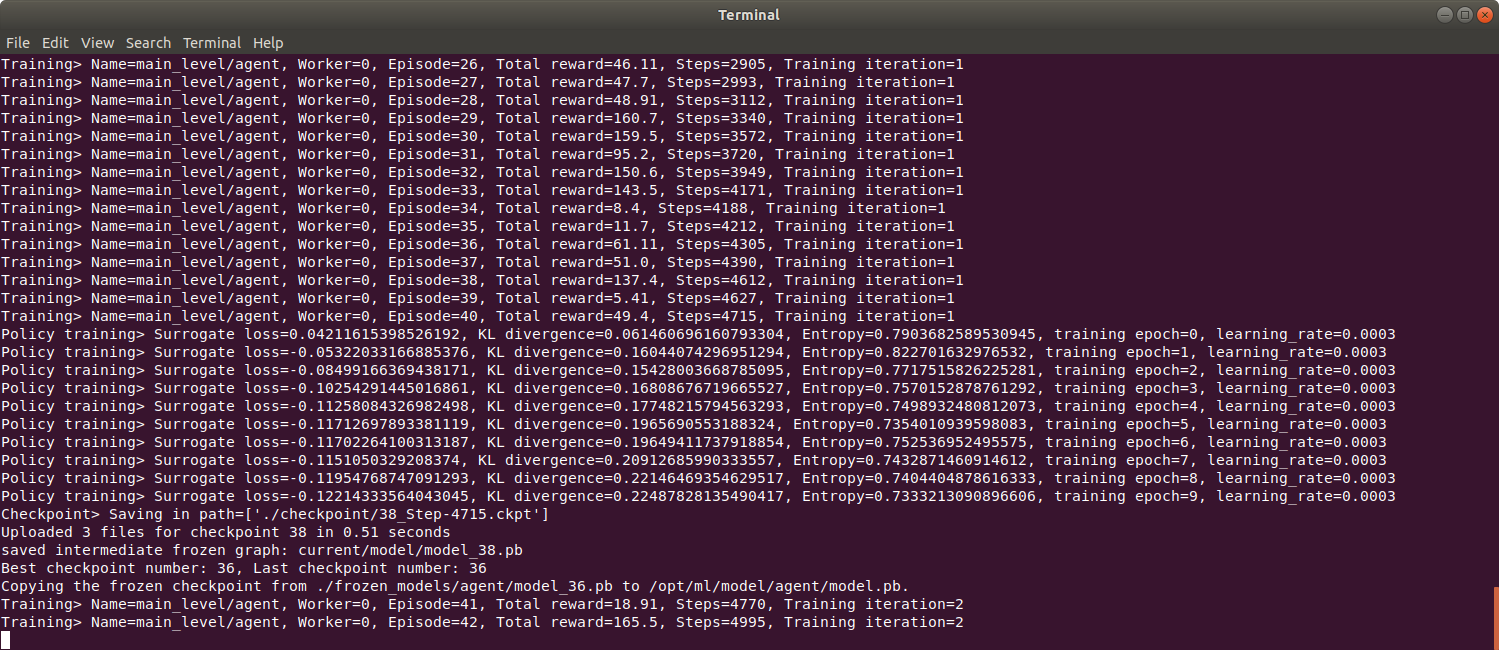
\includegraphics[width=0.9\textwidth]{images/deepracer_local_session1_1_console.png}
    \caption[]{Output from start-training\footnotemark}
    \label{fig:console-output-start}
\end{figure}

If you are complete with the session, use stop-training. This will take approximately 20 - 25s. When the stopping process is completed you should copy your model via local-copy into a save directory. Completing the whole progress you run mk-model an get the finished model, to upload it to your deepracer.

\begin{figure}[H]
    \centering
    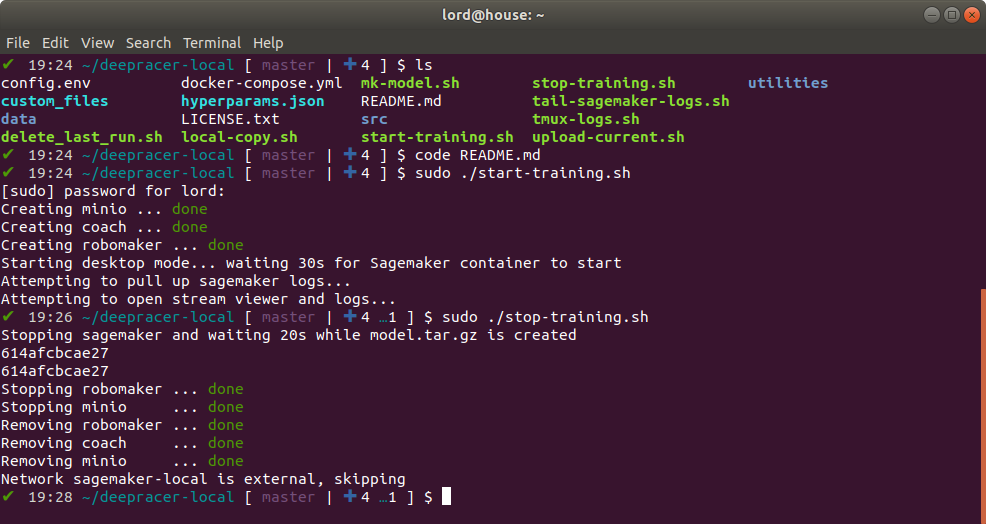
\includegraphics[width=0.9\textwidth]{images/deepracer_local_training_stop.png}
    \caption[]{Output from stop-training\footnotemark}
    \label{fig:console-output-stop}
\end{figure}

\subsection{Uploading a local trained Model}
After finishing a training process you have to upload your model into the Cloud. This is necessary if you want to submit your Model in a Racing League or if you want to evaluate the Training information. Amazon doesnt provide an easy interface to upload data in your model garage.I am going to explain the solution we achived to upload a model in the s3 bucket an use it in your garage.

\begin{enumerate}
    \item At first you have to create a model an train it for at least 5 minutes. This is necessary, because after the training, amazon creates an entry in the s3 bucket, in which all the model information is stored.
    \item The next step is to create the model.tar.gz from your locally trained model. This will be achieved by using mk-model.sh command.
    \item Afterwards you have to copy 
    \begin{itemize}
        \item model-directory
        \item ip-directory
        \item metadata.json
    \end{itemize}
    and swap them with the corresponding directories in the s3 bucket.
    \item At the End you have to navigate back to your model garage and should now be able to evaluate this model. Although the name doesnt change, the metadata and functions should have been swapped.
\end{enumerate}

After an update of the AWS-Console from the 2021-02-22 there is another easier solution:

\begin{enumerate}
    \item You have to use the command mk-model.sh on your pretrained model.
    \item The next step is to navigate into the S3 bucket, create a new Bucket and import the whole folder including:
    \begin{itemize}
        \item model-directory
        \item ip-directory
        \item metadata.json
        \item reward-function.py
    \end{itemize}
    \item Lastly navigate to your model-garage and import the created S3 bucket into the Garage. The Cloud will automatically detect the new model and you can start an evaluation.
\end{enumerate}

\section{Errors occurring during the Installation process}
At our first try we installed all the needed tools and services, but made the mistake to forget to specify the Nvidia CUDA drivers. Although the installation was successful, we were not able to train the model correctly, because the drivers didn't handle the communication between the individual services well. The GUI had a lot of bugs and was mostly unresponsive. We decided to uninstall all the drivers, files and services and get back to 0. We read the instructions one more time slowly and then realised our human error. After repeating the whole installation process but including the wright driver version everything seemed to work fine. 10 minutes into the training process we started receiving python buffer overflow errors, which is very unusual. Debugging the error and reading all log information, we were not able to detect the problem causing the buffer overflow. We gathered information on the internet and came to a conclusion, that the Amazon tools couldn't allocate the memory of the graphics cards properly. Trying out different work-around and solutions we were not able to fix the error or reproduce it in another scenario. After two weeks an a lot of frustrating hours we decided to delete the whole installation and try another different approach. \newline Meanwhile we tried setting up the whole process on our laptops using Ubuntu in an virtual machine. But after discovering the CUDA drivers wouldn't work out of a Virtual Machine because they were not allowed to allocate memory on the physical graphics card, likewise because the hypervisor wouldn't allow that, we tossed out that idea quickly. \newline Another common error we discovered  is that all Repository's rely on the Amazon Tools like Sagemaker and Robomaker, but they dont include the installation in the instructions. You have to read the Ubuntu Wiki and search for the according packages to download.

\section{Difference between Cloud Training and Local Training}
As expected the Local training wasn't performing as good as training in the cloud. In the next section will compare the Hardware and Performance of the PC and the Cloud 

% \subsection{Hardware}

% \subsubsection{PC}

% The local Computer, on which we trained our models consists of

% \begin{table} [H]
% \caption{Computer Components}
% \label{tab:Components}
% \centering
% \setlength{\tabcolsep}{5mm}
% \def\arraystretch{1.25}
% \begin{tabular}{|r|r|c|c|}
% \hline
% \textbf{Hardware} & \textbf{Spec} \\
% \hline\hline
% Processor: & Intel i7 6700k @4GHz \\
% \hline
% Graphics Card: & Nvidia GTX 1070 8gb \\
% \hline
% Memory: & 16gb DDR4 2666MHz \\
% \hline
% \end{tabular}
% \end{table}


% \subsubsection{Amazon Cloud}
% Amazon doesnt provide much Information on its own Hardware, because they change hardware very often and it depends on usage and customer. In our Case research showed that they run


% \begin{table} [H]
% \caption{Amazon Cloud Components}
% \label{tab:Cloud-Components}
% \centering
% \setlength{\tabcolsep}{5mm}
% \def\arraystretch{1.25}
% \begin{tabular}{|r|r|c|c|}
% \hline
% \textbf{Hardware} & \textbf{Spec} \\
% \hline\hline
% Processor: & Dual Socket Intel Xeon E5410 2.33GHz \\
% \hline
% Graphics Card: & unknown \\
% \hline
% Memory: & unknown \\
% \hline
% \end{tabular}
% \end{table}
% \repeatfootcite{Amazon-Cloud-Hardware}
 

\subsection{Performance-Difference}
To exactly measure the difference between the Cloud and the research Computer, we set up a Test-Model. The model specifications are: 
 
\begin{table} [H]
\caption{Sample Model Specifications}
\label{Sample Model Specifications}
\centering
\begin{tabular}{|m{15em}|m{1cm}|}
\hline
\textbf{Hyperparameter} & \textbf{Value} \\
\hline
Gradient descent batch size: & 64 \\
\hline
Entropy: & 0.01 \\
\hline
Discount factor: & 0.999 \\
\hline
Loss type: & Huber \\
\hline
Learning rate: & 0.0003 \\
\hline
Number of experience episodes between each policy-updating iteration: & 20 \\
\hline
Number of epochs: & 10 \\
\hline
\end{tabular}
\end{table}

Using the standard reward function, the model was trained on the Oval Track. We choose this test-environment because its very easy to learn, and only given 30 minutes to train the model, we couldn't train it on a more difficult Track, expecting to master it. Moreover the Race-Mode was set to time-trial, because this model isn't trained to race in a league against other Deepracers.
\newline
To compare the two models, we started an evaluation in the AWS-Cloud. This process simulates the car on the track and drives 3 laps. Then it determines the probability that the deepracer will successfully complete a lap without crossing the line.


\subsubsection{Cloud-Training}
After finishing the Evaluation in the Cloud the Results were:

\begin{figure}[H]
    \centering
    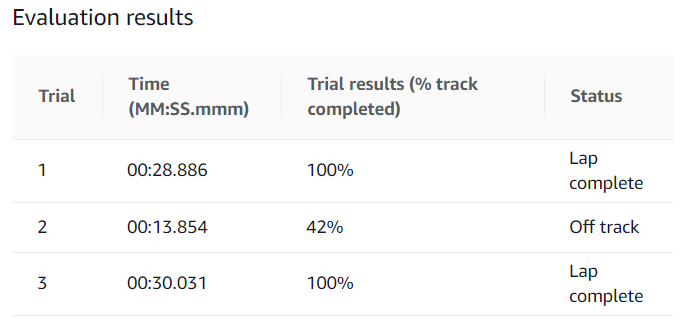
\includegraphics[width=0.9\textwidth]{images/CloudEvaluationResults.PNG}
    \caption[]{Evaluation Results from Cloud Training}
    \label{fig:evRe}
\end{figure}



\subsubsection{Local-Training}
Evaluating the local-Training, the results were as following: 
\begin{figure}[H]
    \centering
    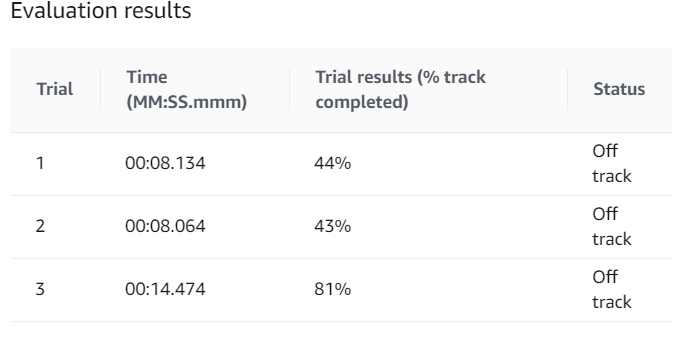
\includegraphics[width=0.9\textwidth]{images/localEvaluation.PNG}
    \caption[]{Evaluation Results from Local Training}
    \label{fig:evLo}
\end{figure}
 
 
\subsection{Price-Difference}
The Table below shows the Difference between storing and evaluating Data online and offline.

\begin{table}[H]
\caption{Pricing for model training with AWS services.}
\label{tab:services}
\centering
\setlength{\tabcolsep}{5mm}
\def\arraystretch{1.25}
\begin{tabular}{|r|r|c|c|}
\hline
\textbf{service} & \textbf{pricing AWS} & \textbf{pricing PC} \\
\hline\hline
training and evaluation & 3.50 US\$ per hour & 0.29 US\$ per Kilowatt per hour \\
\hline
model storage & 0.023 US\$ per GB and month & free of charge\\
\hline
\end{tabular}
\end{table}
\footnote{Cited date 2020/08/20}
\repeatfootcite{PowerCost}

\subsection{Result}
After training in the Cloud and training locally, we came to the conclusion, that the choices depends on the use-case. Comparing the training Data, the Cloud is 40\% faster, otherwise comparing the Cost-Explorer, the Cloud is 1200\% more expensive. The AWS-Management Console has a very detailed documentation and guides that help you creating your first model. Its also very easy and fast to train and evaluate the model. On the other side local training is very cost-efficient although, there is poor to none documentation and if errors occur or, you need to debug you have to have a lot of knowledge of the structure of the Amazon tools and services that are running in the background. 



% If you want an easy and fast way to create, train and evalute models you should remain in the AWS-Management Console. Otherwise if you want to save costs, and got a lot of technical knowledge its better to train local. The Cloud is about 40\% faster and the documentation is very detailed. Training it yourself is a very complicated way to go, that includes a lot of debugging and research. Another prerequisite for local training is to have high performance hardware. 

% \section{Gap to real world environment}



% \section{Deepracer League}

% \subsection{Online-League}

% \subsection{Championships}




% \section{Amazon Management-Console}